\documentclass[9pt]{beamer}
\usepackage{minted}
%\usemintedstyle{manni}
\usemintedstyle{murphy}
\usepackage{hyperref}
\hypersetup{
colorlinks=true,
urlcolor=blue
}
\usepackage{graphicx}

\begin{document}
\title{h5py}
\author{Nick Thompson} 
\date{\today}

\frame{\titlepage}

\begin{frame}[fragile]
\frametitle{Getting started:}
\begin{minted}{bash}
$ git clone https://github.com/NAThompson/h5py_talk.git
$ cd h5py_talk
$ sudo /bin/bash
# docker run -it -v `pwd`:/hdf5_talk /bin/bash
\end{minted}
\end{frame}

\begin{frame}[fragile]
  \frametitle{What is the best scientific data format?}
  \pause
  Compressed CSV.
\end{frame}


\begin{frame}[fragile]
  \frametitle{What is the second best scientific data format?}
  HDF5.
\end{frame}

\begin{frame}[fragile]
  \frametitle{Ever had this conversation?}
  \begin{itemize}
  \item ``These ascii files are too large.''
  \item ``We could use binary.''
  \item ``How long will that take?''
  \item ``4 hours.''
  \item (3 years later . . .) ``WTF!!!''
  \end{itemize}
\end{frame}

\begin{frame}[fragile]
  \frametitle{Edict:}

  Anyone who introduces a custom binary format shall be hanged.
\end{frame}

\begin{frame}[fragile]
  \frametitle{Example:}

  \begin{minted}{bash}
    $ hdfview example_files/compound.h5
  \end{minted}
  \begin{figure}
    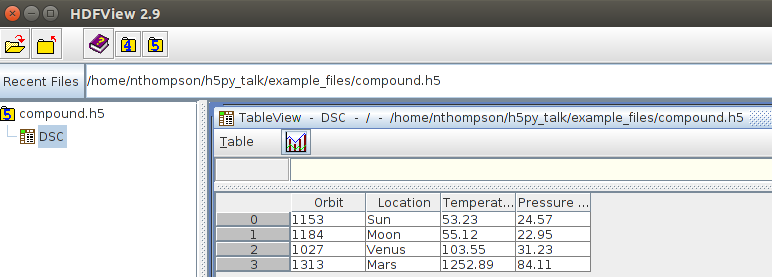
\includegraphics[scale=0.3]{fig/hdfview.png}
  \end{figure}
  \pause
  If you are attempting this in the Docker image, you'll need to set up X-window forwarding.
\end{frame}

\begin{frame}[fragile]
  \frametitle{Explore HDF5 Files}
  \begin{minted}{bash}
    $ h5ls example_files/compound.h5
    $ h5dump example_files/compound.h5
  \end{minted}
\end{frame}


\end{document}
